% Created 2025-09-15 by jos from /l/asm/ and /l/mt/ADCxGather2025.tex

%% \begin{emptyslide}[toc={}]{}
%% %\vspace{\stretch{1}}
%% \vspace{-1.44em}
%% \myFigureRotateToBox{ADCxGather-2025-title-both}{-90}{\twidth}{\theight}{}
%% %\myFigureRotateToBox{ADCxGather-video-zoom-background}{-90}{\twidth}{\theight}{}
%% \vspace{\stretch{1}}
%% \end{emptyslide}

\section[toc={Lightning Hydra Template \emph{Ext}}]{{PyTorch Lightning Hydra Template \emph{Extended} (LHTE)}}

\begin{emptyslide}[toc={}]{}
\vspace{-1.44em}
\myFigureRotateToBox{ADCxGather-2025-title-part1}{-90}{\twidth}{\theight}{}
%\myFigureRotateToBox{ADCxGather-2025-title-LHTE}{-90}{\twidth}{\theight}{}
\vspace{\stretch{1}}
\end{emptyslide}

\begin{slide}[\slideopts,toc={Lightning Hydra Template Ext}]{Lightning Hydra Template Extended (LHTE) --- New Architectures and Datasets}

% ADCxGather2025 abstract 2025-08-24

\vspace{-1em}

% Final onboarding: https://conference.audio.dev/wp-admin/post.php?post=25949&action=edit&var=registration

  \begin{itemize}

    \item Extends the \textbf{Pytorch Lightning + Hydra Template} with top \textbf{image-classification architectures} and \textbf{additional dataset formats}

    \mpitem LHTE began as a fork of the \emph{Lightning Hydra Template (LHT):} \url{https://github.com/ashleve/lightning-hydra-template}
    \begin{itemize}

      \mpitem \emph{PyTorch Lightning} streamlines deep-learning model development in
      numerous ways

      \mpitem \emph{Hydra} is a powerful \emph{configuration management framework} often used

      \mpitem An LHT \emph{example experiment} trains an MLP on MNIST (hand-written digits)

    \end{itemize}

    \mpitem LHTE adds \emph{more architectures:} CNNs,  ViT, ConvNeXt, EfficientNet

    \mpitem LHTE adds \emph{more datasets:} CIFAR-10, CIFAR-100, VIMH:

    \mpitem Variable Image Multi-Head (VIMH) format generalizes CIFAR-100:
    \begin{itemize}
      \mpitem Up to 65k x 65k images with up to 65k channels % NSTM point: (``stacked spectral representations'')
      \mpitem \emph{Multi-Head ready:} Up to 65k \emph{labeled parameters} (8-bit label, 8-bit value)
      \mpitem Example Use: \emph{synthesis parameters} ($\le$ 256 parameters with $\le$ 256 settings each)
      % pairs with \emph{multiple classification / regression heads}
      %% \begin{itemize}
      %%   \mpitem Up to 256 parameters (8 bits)
      %%   \mpitem Up to 256 values for each parameter (8 bits)
      %% \end{itemize}
      \mpitem \emph{Data loaders} for all supported datasets and model architectures
      \mpitem The \texttt{configs/experiment/} directory contains \emph{benchmark replications} % on MNIST, CIFAR, and VIMH datasets
      \mpitem Top-level \texttt{Makefile} contains $\approx 80$ \emph{make targets} for tests, training, experiments
    \end{itemize}
  \end{itemize}

\end{slide}

\begin{slide}[\slideopts,toc={Original LHT}]{Original Lightning Hydra Template (LHT)}

  \emph{Open-Source PyTorch Lightning + Hydra Bootstrap}\\
  \url{https://github.com/ashleve/lightning-hydra-template}

  \begin{itemize}
    \mpitem PyTorch \emph{project skeleton} with \texttt{src/}, \texttt{configs/}, and \texttt{tests/}, ready for research

    \mpitem \emph{Chatbots love it} % (They've probably seen a lot of it)

    \mpitem \emph{Hydra workflow:} CLI overrides such as:\\
    \hspace{0.1em}\texttt{> python src/train.py trainer=gpu data.batch\_size=64}\\
    for every configuration value ($\approx 300$ --- thousands in the LHTE)
    % LHTE: (19,402 at last count: 2,383 in the main \texttt{configs/})

    \mpitem \emph{PyTorch Lightning baseline:} single-head MNIST MLP experiment --- \emph{that's it!} % , reproducible training loops, and logging hooks

    \mpitem \emph{Make targets} for testing, training, and admin % , Conda or pip installation paths, and template README for new repos

    \mpitem LHTE maintains \emph{compatibility} with existing LHT configs, datasets, and checkpoints

  \end{itemize}

\end{slide}

%% Nice intro slide from the new GPT5-Codex, but covered already:
%% \begin{slide}[\slideopts,toc={Why LHTE}]{Why Lightning Hydra Template \emph{Extended}?}
%%   \emph{Motivation:}
%%   \begin{itemize}
%%     \mpitem Beyond MLP, integrate SimpleCNN, ConvNeXt-V2, EfficientNet, ViT, SDN, and multihead MLPs ship side by side
%%     \mpitem Out-of-the-box datasets beyond MNIST: CIFAR-10/100, multihead synth suites, and the new Variable Image MultiHead (VIMH) format
%%     \mpitem Hydra-first overrides encourage rapid prototyping --- swap data, models, trainers, and losses without touching code
%%     \mpitem Developer ergonomics matter: 100+ make targets, scripted smoke tests, and diagram tooling keep the feedback loop tight
%%     \mpitem Everything remains compatible with upstream LHT so existing configs and checkpoints keep working
%%   \end{itemize}
%% \end{slide}
%%
%% Ditto - this was written from an intro to the code, so more aimed at that:
%% \begin{slide}[\slideopts,toc={LHTE Tour}]{LHTE in 5 Minutes}
%%   \emph{Hands-On Preview}
%%   \begin{itemize}
%%     \mpitem \texttt{bash setup.bash} to bootstrap a uv-managed virtual environment with PyTorch + Lightning
%%     \mpitem \texttt{make h} surfaces discoverable commands; \texttt{make tqa} runs MNIST smoke trains across every architecture
%%     \mpitem CIFAR baselines: \texttt{make cbqa} (quick sanity), \texttt{make cbs10/cbs100} (full benchmarks with logs)
%%     \mpitem Real multihead workloads: \texttt{python src/train.py experiment=vimh\_cnn} auto-configures heads from dataset metadata
%%     \mpitem Mix and match with CLI overrides such as \texttt{trainer.max\_epochs=1} or \texttt{model.loss=focal} to explore variants
%%   \end{itemize}
%% \end{slide}
%%
%% \begin{slide}[\slideopts,toc={Feature Map}]{Feature Map \& Documentation Trail}
%%   \emph{Where to Dive Deeper}
%%   \begin{itemize}
%%     \mpitem Architectures roundup: \texttt{docs/architectures.md} for parameter counts, diagrams, and recommended use cases
%%     \mpitem Dataset guide: \texttt{docs/vimh.md} + \texttt{docs/vimh\_cookbook.md} explain the metadata schema and sampling recipes
%%     \mpitem Benchmark ledger: \texttt{docs/benchmarks.md} documents CIFAR + VIMH comparisons with reproducible Hydra configs
%%     \mpitem Multihead strategy: \texttt{docs/multihead.md} covers head wiring, loss combinations, and evaluation metrics
%%     \mpitem Vision primer handout: \texttt{docs/vision\_primer.md} mirrors these slides for quick sharing without LaTeX
%%   \end{itemize}
%% \end{slide}
%%
%% Actually notes to ME:
%% \begin{slide}[\slideopts,toc={Talk Flow}]{Suggested Talk Flow}
%%   \emph{Use LHTE to Frame Your Story}
%%   \begin{itemize}
%%     \mpitem Start with the Lightning + Hydra reuse pitch, then highlight how LHTE supercharges it with modern backbones
%%     \mpitem Walk through the architecture menu and pair each backbone with a ready-to-run experiment
%%     \mpitem Demo quick wins: smoke tests, CIFAR comparisons, and VIMH runs with a few terminal commands
%%     \mpitem Land on multihead motivation and roadmap --- point to benchmark snapshots and upcoming extensions
%%     \mpitem Close by inviting the audience to clone the repo, open \texttt{docs/index.md}, and follow the handout for self-serve exploration
%%   \end{itemize}
%% \end{slide}

\section[toc={New Architectures}]{LHTE Architectures: MLP += \\
  CNNs + ViT + ConvNeXt + EfficientNet}

\begin{slidewhite}[\slideopts,toc={CNN}]{SimpleCNN Architecture}

  \centerline{
\includegraphics[width=\textwidth]{cnn_architecture.eps}}

  \emph{Convolutional Neural Network for Spatial Feature Extraction}

  \begin{itemize}
    \mpitem MNIST and CIFAR-10/100 benchmark examples included, e.g.:

    \mpitem \emph{Two conv layers:} 3×3 kernels, 32→64 channels, MaxPool, BatchNorm

    \mpitem \emph{Adaptive pooling:} 7×7 feature maps → FC classifier with dropout

    \mpitem \emph{Parameter variants:} 8K (small), 68K (medium), 421K (large):\\
    \texttt{./configs/mnist\_cnn\_[8k|68k|421k].yaml}

    \mpitem \emph{Performance:} CIFAR-10: 85-92\%, CIFAR-100: 55-70\%

    \mpitem Supports multihead classification for multi-task learning
  \end{itemize}

\end{slidewhite}

\begin{wideslide}[\slideopts,toc={YAML},method=direct]{LHTE Architecture Config Files}
{\footnotesize
\begin{verbatim}
cifar10_cnn_medium.yaml         cifar100_efficientnet_210k.yaml    mnist_efficientnet_22k.yaml
cifar10_convnext_128k.yaml      cifar100_sdn_1m.yaml               mnist_efficientnet_7m.yaml
cifar10_convnext_210k.yaml      cifar100_vit_210k.yaml             mnist_mh_cnn_422k.yaml
cifar10_convnext_medium.yaml    cifar100mh_cnn_medium.yaml         mnist_sdn_68k.yaml
cifar10_efficientnet_210k.yaml  cifar100mh_convnext_210k.yaml      mnist_sdn_8k.yaml
cifar10_mh_cnn_medium.yaml      cifar100mh_efficientnet_210k.yaml  mnist_vit_210k.yaml
cifar10_vit_210k.yaml           cifar100mh_vit_210k.yaml           mnist_vit_38k.yaml
cifar100_cnn_1m_original.yaml   mnist_cnn_421k.yaml                mnist_vit_821k.yaml
cifar100_cnn_1m.yaml            mnist_cnn_68k.yaml                 mnist_vit_995.yaml
cifar100_cnn_medium.yaml        mnist_cnn_8k.yaml                  mnist_vit_pytorch.yaml
cifar100_coarse_cnn_medium.yaml mnist_convnext_210k.yaml           multihead.yaml
cifar100_convnext_10m.yaml      mnist_convnext_68k.yaml            vimh_cnn_medium_ordinal.yaml
cifar100_convnext_1m.yaml       mnist_convnext_821k.yaml           vimh_cnn_medium_regression.yaml
cifar100_convnext_210k.yaml     mnist_convnext_8k.yaml             vimh_cnn_medium.yaml
\end{verbatim}
}
\textbf{LHT:} \; \texttt{example.yaml}
\end{wideslide}

\begin{slide}[\slideopts,toc={ConvNeXt}]{ConvNeXt-V2 Architecture}

  \centerline{\includegraphics[width=\textwidth]{convnext_architecture.eps}}

  \emph{Modern CNN with Global Response Normalization (GRN)}

  \begin{itemize}
    \item \emph{Key innovation:} GRN normalizes across spatial/channel dimensions

    \item \emph{Architecture:} 7×7 depthwise conv, LayerNorm, 4× MLP with GELU

    \item \emph{Sizes:} Tiny (18K), Small (73K), Base (288K), Large (725K)

    \item \emph{Best performer:} CIFAR-10: 90-95\%, CIFAR-100: 70-80\%
  \end{itemize}

\end{slide}

\begin{slide}[\slideopts,toc={EfficientNet}]{EfficientNet Architecture}

  \centerline{\includegraphics[width=1.1\textwidth]{efficientnet_architecture.eps}}

  \emph{Optimized CNN for Mobile and Edge Deployment}

  \begin{itemize}
    \item \emph{Compound scaling:} Balances depth, width, and resolution

    \item \emph{Mobile-optimized:} Inverted residuals, squeeze-excitation, Swish

    \item \emph{Sizes:} 22K (edge), 210K (balanced), 7M (high accuracy)

    \item \emph{Performance:} CIFAR-10: 89-94\%, CIFAR-100: 67-77\%
  \end{itemize}

\end{slide}

\begin{slide}[\slideopts,toc={ViT}]{Vision Transformer (ViT) Architecture}

  \centerline{
\includegraphics[width=1.1\textwidth]{vit_architecture.eps}}

  \emph{Attention-Based Learning on Image Patches}

  \begin{itemize}
    \item \emph{Image → Patches:} 28×28 → 7×7 patches → token sequence

    \item \emph{Self-attention:} Multi-head attention + MLP with GELU

    \item \emph{Sizes:} Tiny (38K), Small (210K, MNIST SOTA: 99.5\%), Base (821K)

    \item Highly parallelizable, scales with data and compute
  \end{itemize}

\end{slide}

\section[toc={New Dataset Formats}]{Datasets Beyond MNIST}

\begin{slide}[\slideopts,toc={CIFAR-10}]{CIFAR-10 Dataset Support}

  \centerline{\includegraphics[width=0.6\textwidth]{cifar10_samples.eps}}

  \emph{Standard Computer Vision Benchmark}

  \begin{itemize}
    \item 10 classes, 32×32 RGB, 50K train / 10K test

    \item \emph{LHTE Results:}
    %% \begin{itemize}
    %%   \item CNN (85-92\%)
    %%   \item ConvNeXt (90-95\%)
    %%   \item ViT (88-93\%)
    %% \end{itemize}
    \item \emph{LHTE Results:} CNN (85-92\%), ConvNeXt (90-95\%), ViT (88-93\%)

    \item \emph{Commands:} \texttt{make cbq10c} (quick), \quad \texttt{make cb10c} (full)

    \item Literature-competitive performance out-of-the-box
  \end{itemize}

\end{slide}

\begin{slide}[\slideopts,toc={CIFAR-100}]{CIFAR-100 Dataset Support}

  \centerline{\includegraphics[width=0.7\textwidth]{cifar100_samples.eps}}

  \emph{Fine-Grained Classification Challenge}

  \begin{itemize}
    \item 100 fine classes or 20 coarse superclasses, 32×32 RGB

    \item \emph{Performance:} ConvNeXt leads at 70-80\% (fine), 85\% (coarse)

    \item \emph{Multihead:} Simultaneous fine + coarse classification

    \item \emph{Commands:} \texttt{make cb100c}, \quad \texttt{make cbs100}

  \end{itemize}

\end{slide}

\begin{slidewhite}[\slideopts,toc={VIMH}]{Variable Image MultiHead (VIMH) Format}
  \vspace{-2.5em}
  \myFigureRotateToBox{vimh-proj}{-90}{\twidth}{0.45\theight}{}

  \vspace{-0.5em}
  \emph{Generalized Dataset Format for Multi-Parameter Learning}
  \vspace{-0.5em}

  \begin{itemize}
    \mpitem \emph{Self-describing:} Variable dimensions up to 65k×65k×65k (16-bit metadata)

    \mpitem \emph{Flexible labels:} 0-255 parameters, 8-bit quantized (~100 steps)

    \mpitem \emph{Per sample:} [height, width, channels] + [N params] + [ID,val pairs] + image

    \mpitem \emph{Applications:} Audio spectrograms, vision, scientific data

    \mpitem Models auto-configure from dataset metadata
  \end{itemize}
\end{slidewhite}

%% \begin{slide}[\slideopts,toc={}]{Variable Image MultiHead (VIMH) Format}
%%   \centerline{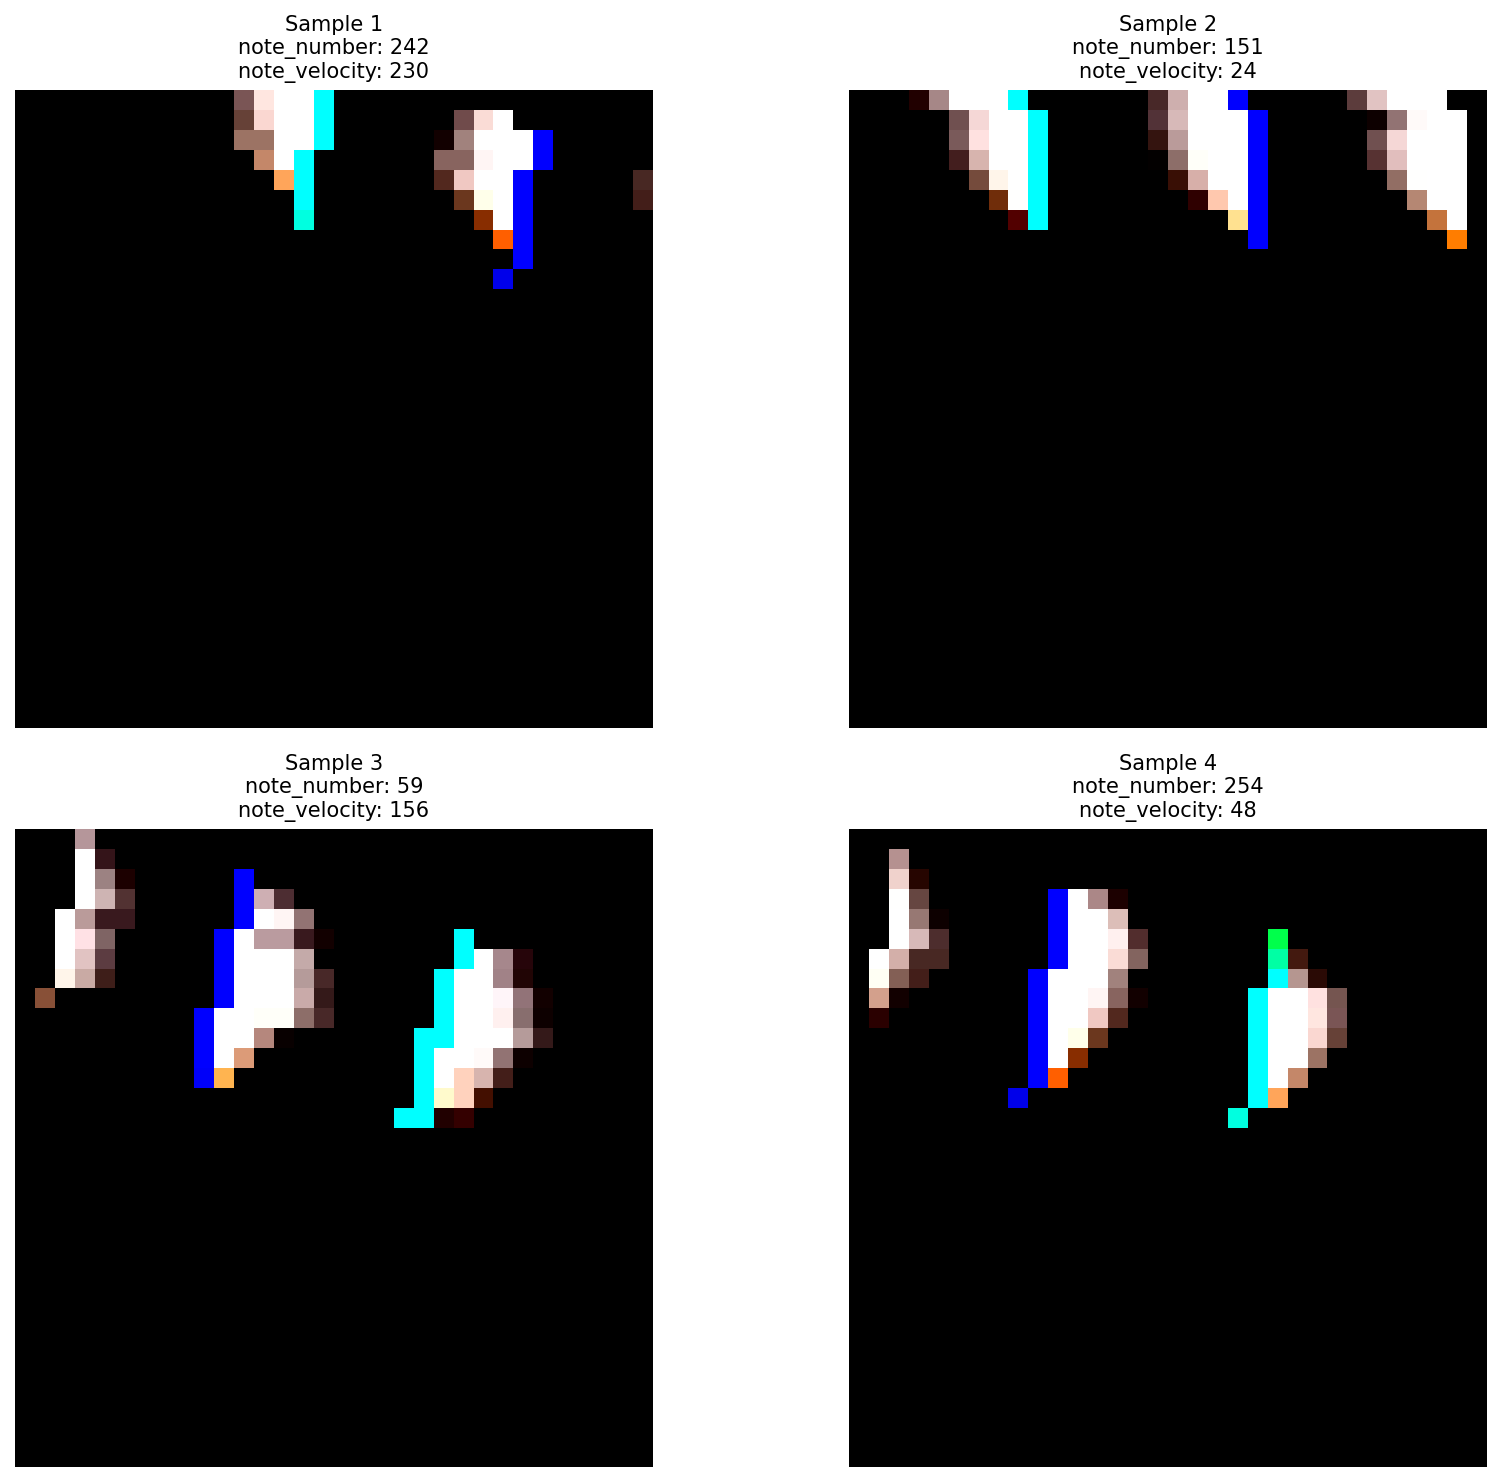
\includegraphics[width=0.9\textwidth]{png/sample_data.eps}}
%% \end{slide}


\begin{slide}[\slideopts,toc={MultiHead}]{Multi-Head Classification Support}

  \vspace{-1em}

  % \centerline{
\includegraphics[width=0.5\textwidth]{viz/diagrams/multihead_architecture.eps}}
  \scalebox{0.7}{
    \input multihead.tex
  }

  \emph{Training Networks with Multiple Output Tasks}

  \begin{itemize}
    \mpitem \emph{Architecture:} Shared backbone → separate heads per task

    \mpitem \emph{Task types:} Classification, ordinal regression, pure regression

    \mpitem \emph{Examples:} MNIST (digit+thickness), CIFAR-100 (fine+coarse),\\
    VIMH (synthesis-parameter + parameter-value)

    \mpitem Configurable via Hydra without code changes
  \end{itemize}
\end{slide}
%% \begin{slide}[\slideopts,toc={}]{Multi-Head Classification Support}
%%   \scalebox{1.0}{
%%     \input multihead.tex
%%   }
%% \end{slide}

\begin{slide}[\slideopts,toc={Benchmarks}]{Benchmark Replications \& Experiments}

  \emph{$\approx 30$ Pre-Configured Experiments}

  \begin{itemize}
    \mpitem \emph{Categories:} MNIST, CIFAR-10/100, VIMH, Multihead

    \mpitem \emph{Features:} Fixed seeds, fair comparisons, automated tracking

    \mpitem \emph{Example Make Commands} (abbreviated and full):
    \begin{itemize}
      \mpitem \texttt{make ca} \quad \quad (or \texttt{make compare-arch})
      \mpitem \texttt{make cbqa} \quad (or \texttt{make cifar-benchmark-quick-all})
      \mpitem \texttt{make cbsa} \quad (or \texttt{make cifar-benchmark-suite-all})
    \end{itemize}
    \mpitem Version-controlled experiment configs ensure reproducibility
  \end{itemize}
\end{slide}

\begin{wideslide}[\slideopts,toc={Experiments},method=direct]{LHTE Experiment Config Files}
{\footnotesize
\begin{verbatim}
cifar10_benchmark_cnn.yaml            cifar100_cnn.yaml             multihead_cnn_cifar10.yaml
cifar10_benchmark_convnext.yaml       cifar100_coarse_cnn.yaml      multihead_cnn_mnist.yaml
cifar10_benchmark_efficientnet.yaml   cifar100mh_cnn.yaml           vimh_cnn_16kdss_ordinal.yaml
cifar10_benchmark_vit.yaml            cifar100mh_convnext.yaml      vimh_cnn_16kdss_regression.yaml
cifar10_cnn_cpu.yaml                  cifar100mh_efficientnet.yaml  vimh_cnn_16kdss.yaml
cifar10_cnn.yaml                      cifar100mh_vit.yaml           vimh_cnn.yaml
cifar10_convnext_128k_optimized.yaml  cnn_mnist.yaml                vit_mnist_995.yaml
cifar10_convnext_medium_optimized.yaml convnext_mnist.yaml           vit_mnist.yaml
cifar100_benchmark_cnn.yaml           convnext_v2_official...
cifar100_benchmark_convnext.yaml      example.yaml
\end{verbatim}
}
\textbf{LHT:} \; \texttt{mnist.yaml}
\end{wideslide}

%% TOO DOWN IN THE WEEDS
%% \begin{slide}[\slideopts,toc={Makefile}]{$\approx 80$ Makefile Targets}
%%   \emph{Streamlined Research Workflow}
%%   %% \begin{itemize}
%%   %%   \mpitem \emph{Abbreviations:} \texttt{t*} (train), \texttt{tq*} (quick), \texttt{cb*} (CIFAR), \texttt{e*} (experiments)
%%   %%   \mpitem \emph{Progressive testing:} \texttt{tq} → \texttt{ca} → \texttt{cbqa} → \texttt{cbs}
%%   %%   \mpitem \emph{Productivity:} \texttt{make help}, logical naming, batch operations
%%   %% \end{itemize}
%% \end{slide}

\papersection{Future Work}{

  Next Steps:
  \begin{itemize}
  \item Merge PRs
  \item Chatbot Reviews (GPT, Claude, Gemini, \dots)
  \end{itemize}

  \vspace{2em}

  \centerline{
\includegraphics[width=2cm]{eps/lhte_qr_code.eps}}
  \vspace{2pt}
  \centerline{{\scriptsize github.com/josmithiii/lightning-hydra-template-extended}}
}

\begin{slide}[\slideopts,toc={}]{Summary of Resources Online}
  \begin{itemize}
    \item \emph{Neural Spectral Modeling Template (NSMT):}\\
      \href{https://github.com/josmithiii/neural-spectral-modeling-template.git}
           {\texttt{github.com/josmithiii/neural-spectral-modeling-template}}
    \item[]
    \item \emph{Lightning Hydra Template Extended (LHTE):}\\
      \href{https://github.com/josmithiii/lightning-hydra-template-extended.git}
           {\texttt{github.com/josmithiii/lightning-hydra-template-extended}}
    \item[]
    \item \emph{Lightning Hydra Template (LHT):}\\
      \href{https://github.com/ashleve/lightning-hydra-template}
           {\texttt{github.com/ashleve/lightning-hydra-template}}
    \item[]
    \item JOS Home Page (Videos, Overheads, including these):\\
      \href{https://ccrma.stanford.edu/~jos/Welcome.html}
           {\texttt{https://ccrma.stanford.edu/\~{}jos/}}
  \end{itemize}
\end{slide}
